\tikzset{every picture/.style={line width=0.75pt}} %set default line width to 0.75pt        

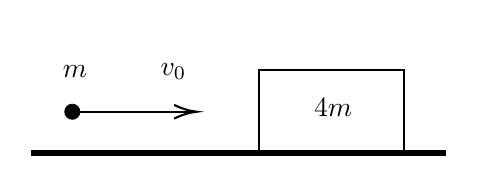
\begin{tikzpicture}[x=0.75pt,y=0.75pt,yscale=-1,xscale=1]
%uncomment if require: \path (0,284); %set diagram left start at 0, and has height of 284

%Straight Lines [id:da2354228935219831] 
\draw [line width=2.25]    (250,170) -- (450,170) ;
%Straight Lines [id:da4423200662416875] 
\draw    (270,150) -- (328,150) ;
\draw [shift={(330,150)}, rotate = 180] [color={rgb, 255:red, 0; green, 0; blue, 0 }  ][line width=0.75]    (10.93,-3.29) .. controls (6.95,-1.4) and (3.31,-0.3) .. (0,0) .. controls (3.31,0.3) and (6.95,1.4) .. (10.93,3.29)   ;
\draw [shift={(270,150)}, rotate = 0] [color={rgb, 255:red, 0; green, 0; blue, 0 }  ][fill={rgb, 255:red, 0; green, 0; blue, 0 }  ][line width=0.75]      (0, 0) circle [x radius= 3.35, y radius= 3.35]   ;
%Shape: Rectangle [id:dp013730634635779948] 
\draw   (360,130) -- (430,130) -- (430,170) -- (360,170) -- cycle ;
%Straight Lines [id:da8167829398208026] 
\draw [draw opacity=0][fill={rgb, 255:red, 255; green, 255; blue, 255 }  ,fill opacity=1 ]   (250,110) -- (450,110) ;

% Text Node
\draw (385,142.4) node [anchor=north west][inner sep=0.75pt]    {$4m$};
% Text Node
\draw (264,126.4) node [anchor=north west][inner sep=0.75pt]    {$m$};
% Text Node
\draw (311,125.4) node [anchor=north west][inner sep=0.75pt]    {$v_{0}$};

\end{tikzpicture}